\section{Design}
\label{sec:design}

Motivated by state-of-the-art tools' inflexibility to change their preemption points,
we introduce a new technique called {\em Iterative Deepening} for adjusting the preemption points at runtime.
Named after the analogous technique in chess artificial intelligence \cite{iterative-deepening-chess-ai},
this approach likewise makes progressively deeper searches of the state space until a given CPU budget is exhausted.
Rather than attempting to search a single state space with every available preemption point enabled
(e.g., preempting on every pthread API call),
Iterative Deepening searches among different combinations of such points during the test,
deciding on-the-fly whether to pursue each resulting state space, or to defer it in favour of smaller ones.
Different state spaces are generated based on {\em subsets} of the preemption points which prior work would use; for example, ``preempt on all calls to {\tt mutex\_lock} but not on {\tt mutex\_unlock}''.
We show a visualization in Figure~\ref{fig:id}.

\begin{figure}[t]
	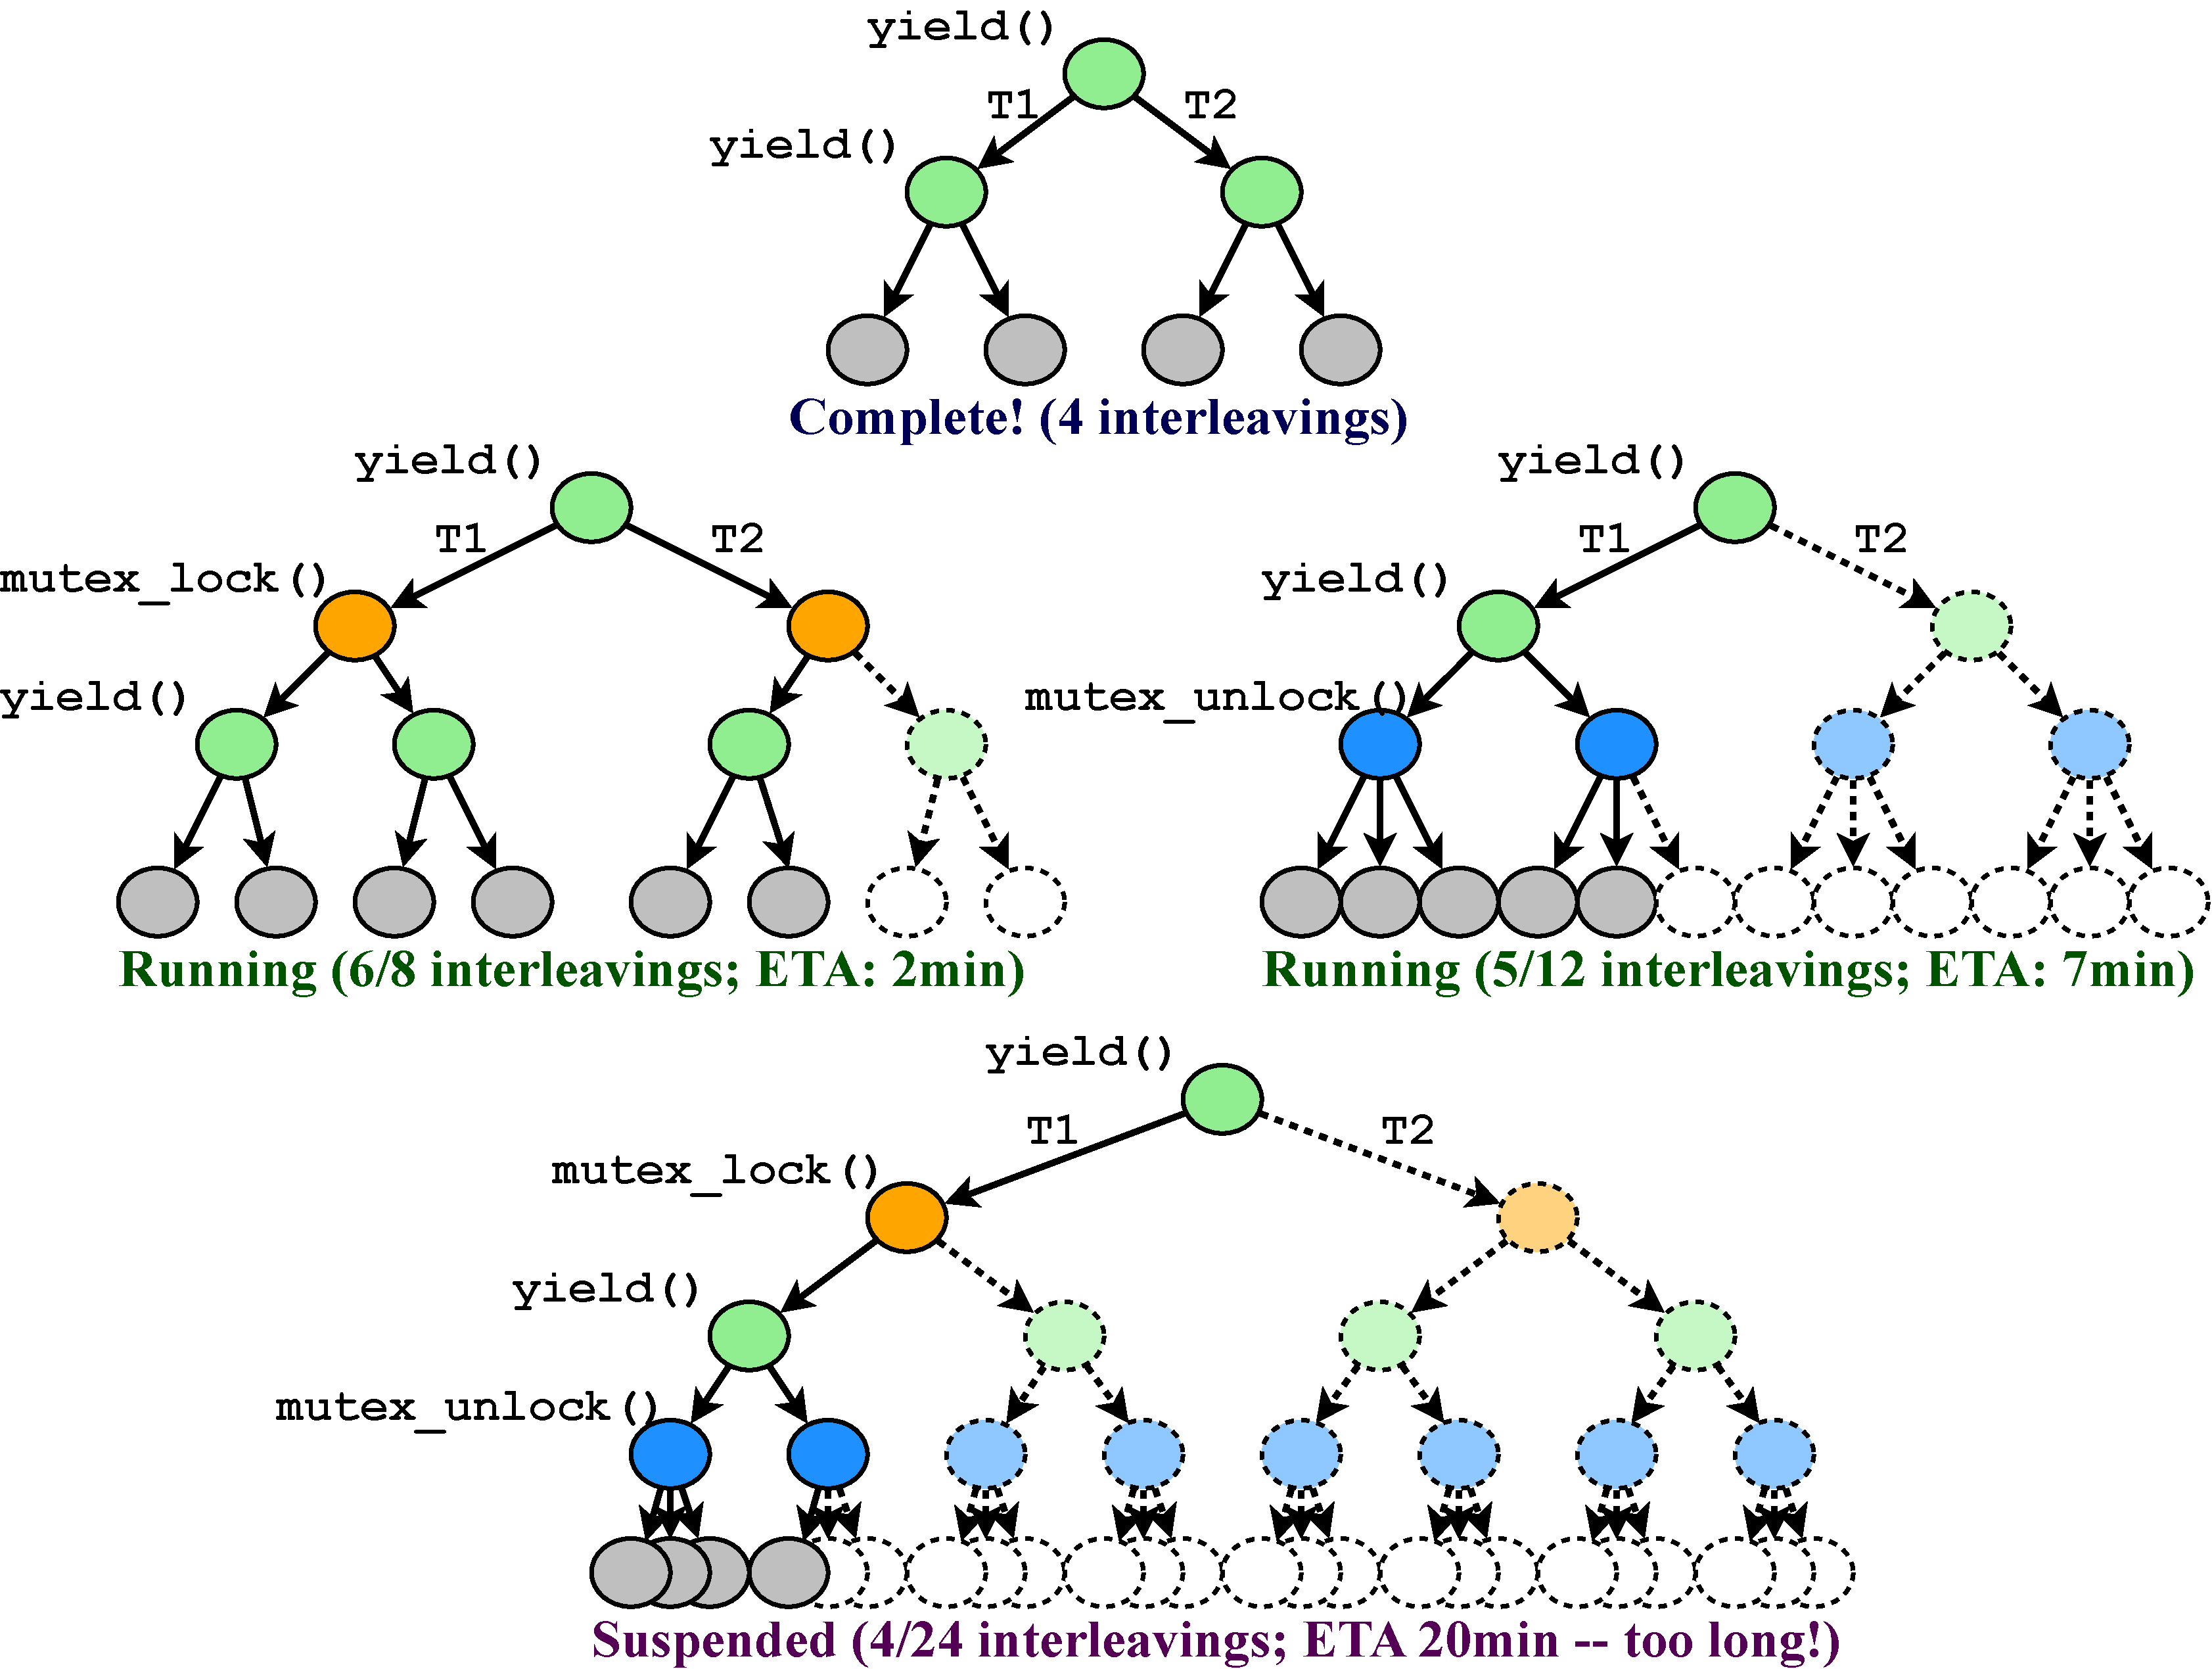
\includegraphics[width=0.48\textwidth]{trees.pdf}
	%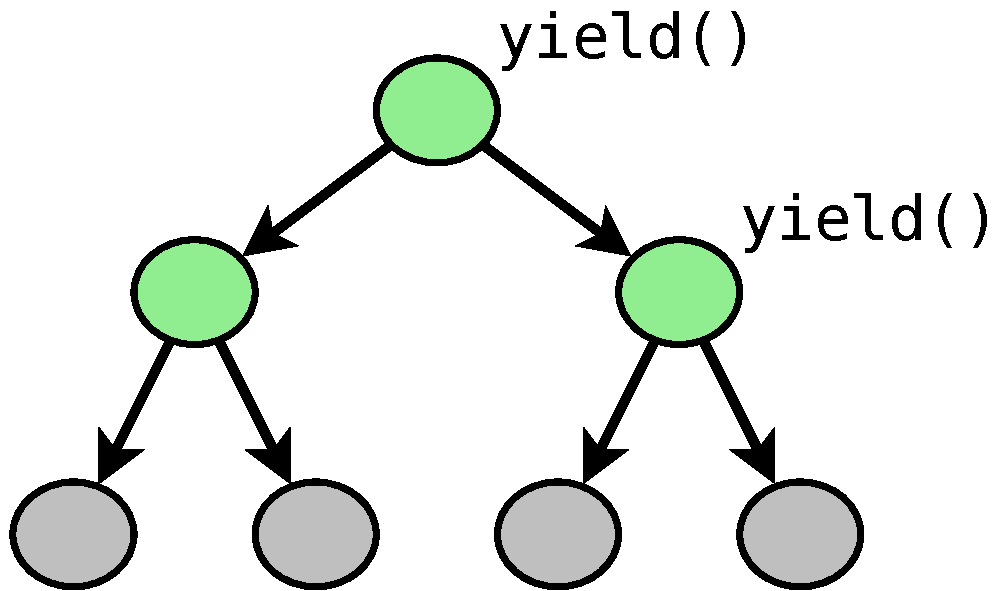
\includegraphics[width=0.15\textwidth]{tree0.pdf}
	%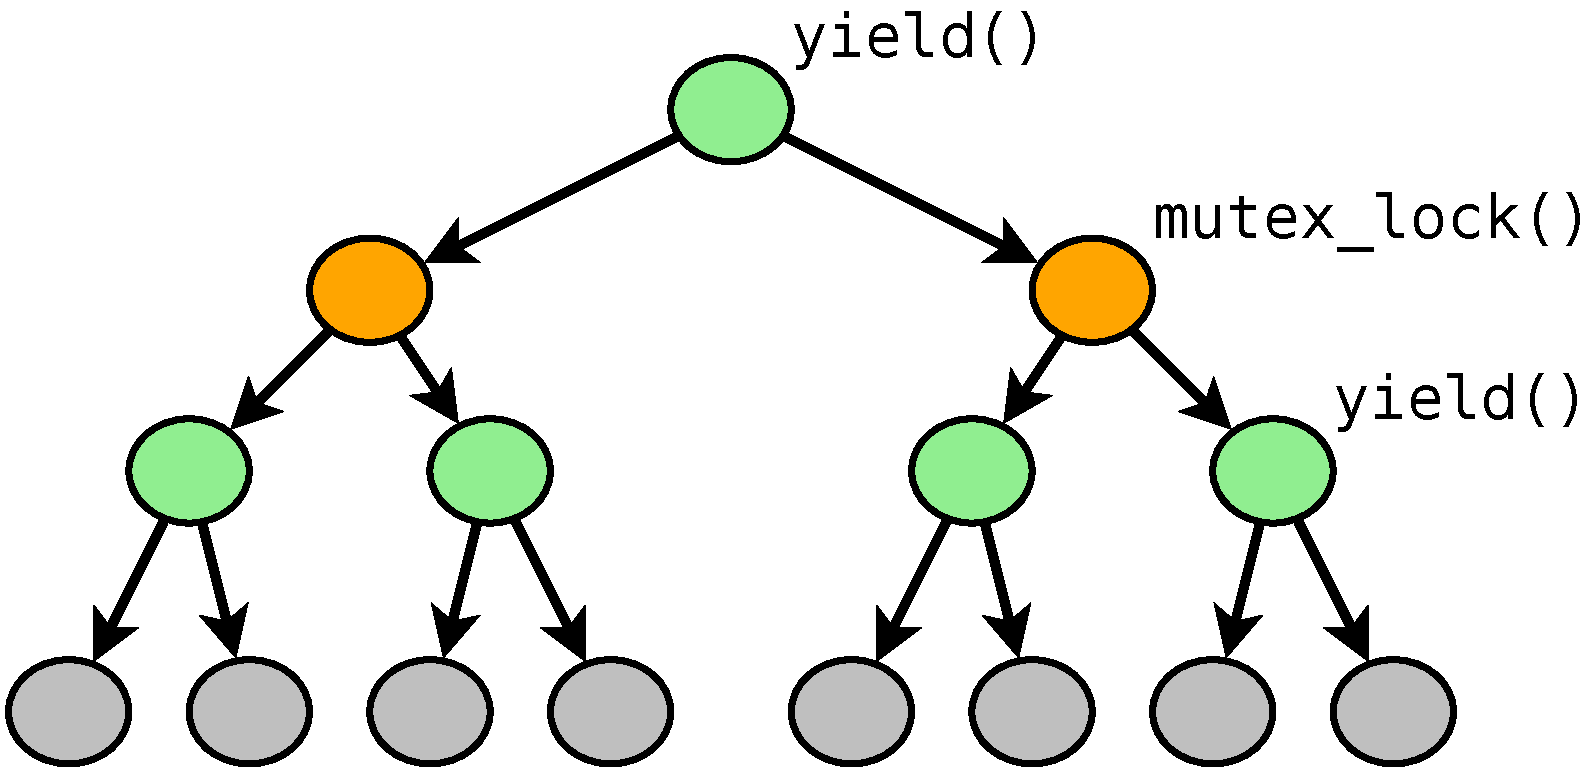
\includegraphics[width=0.225\textwidth]{tree1.pdf}
	%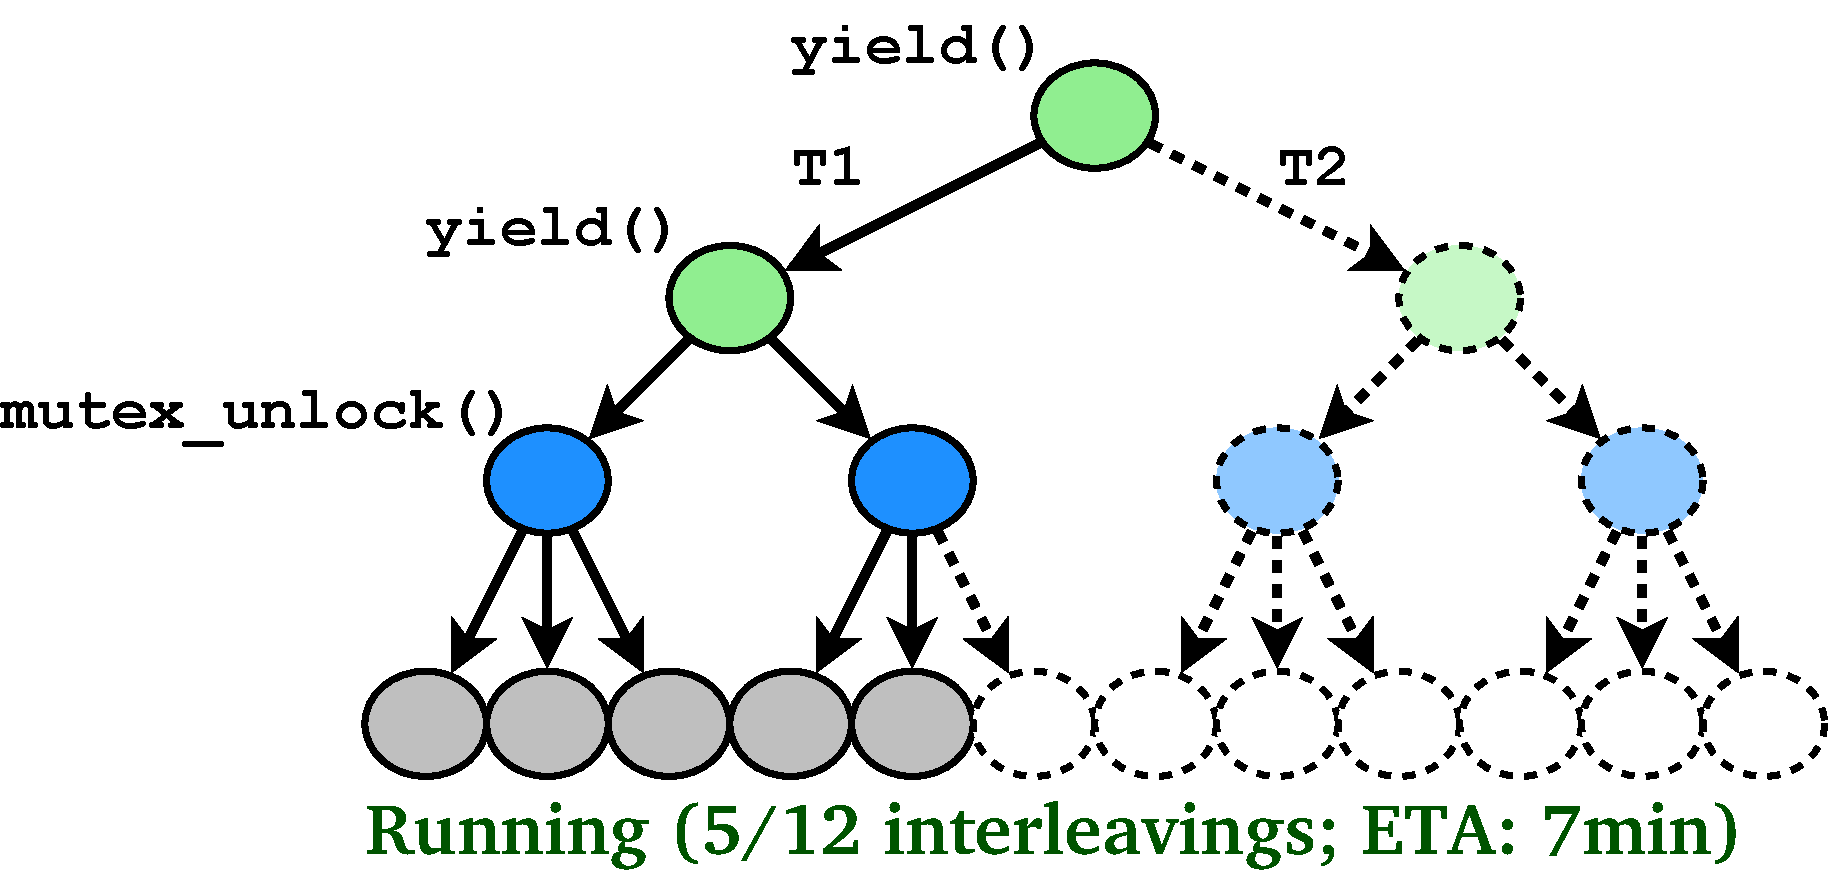
\includegraphics[width=0.25\textwidth]{tree2.pdf}
	%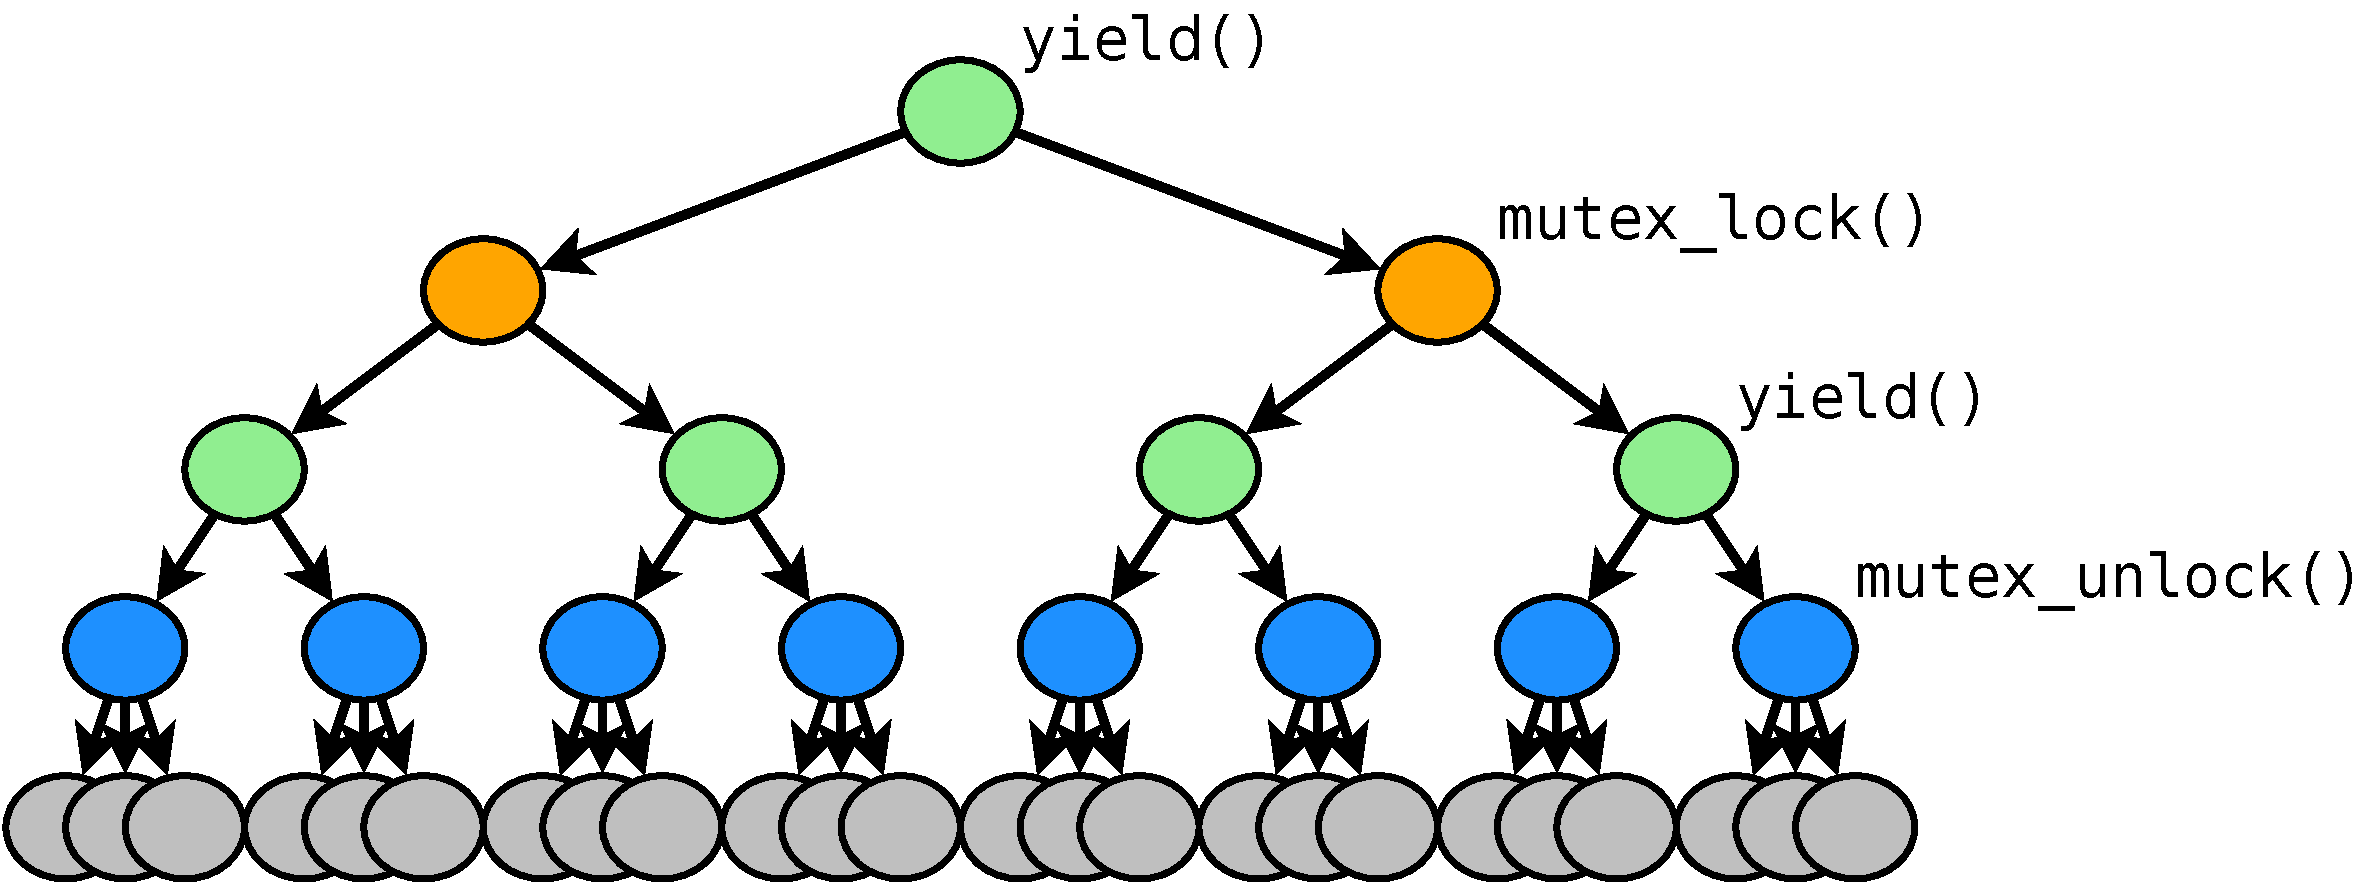
\includegraphics[width=0.35\textwidth]{tree3.pdf}
	\caption{Iterative Deepening example.
		The minimal state space (top) includes only voluntary thread switches, such as {\tt yield()}. %or {\tt cond\_wait()}.
		Multiple further tests can be run: preempting on calls to {\tt mutex\_lock} alone (left), {\tt mutex\_unlock} alone (right), or both together (bottom).
Each option increases the state space size by an unpredictable factor, so multiple state spaces should be tested in parallel.
Estimation techniques~\cite{estimation} inform which state spaces to prioritize.
}
	\label{fig:id}
\end{figure}

Iterative Deepening relies on state-space estimation \cite{estimation}
to understand which state spaces are likely to complete on time,
in advance of actually testing each interleaving within.
The purpose is to make decisions automatically about when to defer exploration of a state space,
so an inexpert user must provide only their total CPU budget as a test parameter,
and to enable completing appropriately-sized state spaces within that budget.

Note that Iterative Deepening is a {\em wrapper} algorithm around stateless model checking.
A model checking tool is still used to test each state space, and other reduction techniques are still applicable.
Moreover, because Iterative Deepening treats the set of preemption points as mutable,
it can add new ones reactively based on any runtime analysis.
In this paper we focus on dynamic data-race detection~\cite{tsan} as the mechanism for finding new preemption candidates.

\subsection{Terminology}

For the rest of the paper, we will abbreviate {\em preemption point} (PP),
%For the remainder of the paper, we will abbreviate {\em preemption point} (PP),
{\em model checking} (MC),
{\em single-state-space model checking} (SSS-MC), % (i.e., the approach of prior work),
Dynamic Partial Order Reduction (DPOR), and {\em state space estimate} (ETA).

SSS-MC indicates the approach of prior model checking tools:
the set of PPs is fixed in advance, and the tool commits to testing every interleaving available with those PPs.
%Reduction techniques are often used to skip equivalent interleavings \cite{dpor}, and search-ordering strategies
Many techniques exist to skip equivalent interleavings and order the search to uncover bugs faster \cite{dpor,demeter,chess-icb,gambit},
but new PPs cannot be added, nor ineffective ones removed, by any dynamic analysis.

We distinguish between data-race {\em candidates} and data-race {\em bugs}.
Because data-race analysis is prone to false-positives,
we classify unprotected access pairs separately from concrete observable failures, % "concrete"?
calling such pairs {\em data race candidates}.
Should a future interleaving, preempting during those accesses,
% TODO: joshua wants 'failure' to be explicitly defined
lead to a failure (e.g. assertion or deadlock), then we report a {\em data-race bug}.
Otherwise, if the access pair can be reordered, but does not produce a failure under any interleaving, it is a {\em benign data race}.
If they cannot be reordered at all, it is a {\em false positive}.
%TODO: Don't do this, below. Scan paper for uses of 'false positive' where you mean to say 'benign' or 'both'.
%For brevity, we count benign data races as a subset of false positives.

We also identify the {\em minimal} and {\em maximal state space} for each test.
The {\em minimal state space} includes only thread switches arising from normal execution (Figure~\ref{fig:id}).
The {\em maximal state space} is simply the one explored by SSS-MC: all statically-available PPs are enabled.
%However, should new data-race PPs be added during a test, the new maximal state space will be the one including those as well.
%% don't say this ^ -- because when you add dr pps, they add in pairs and there would be multiple maximals, at least until they each get explored and subseuqnetly add a pp of the other of the pair.

\subsection{Choosing the best job}

\newcommand\PendingJobs{\ensuremath{\mathcal{P}}}
\newcommand\SuspendedJobs{\ensuremath{\mathcal{S}}}
\newcommand\GetETA[1]{ETA(#1)}
\newcommand\GetPPSet[1]{PPSet(#1)}
With a limited CPU budget, we must avoid running tests that are likely to be fruitless.
Hence, we separate the available PP sets into a set of {\em suspended} jobs (partially-explored state spaces with high ETAs),
and a set of {\em pending} jobs (untested ones with unknown ETAs).
When a MC instance reports an ETA too high,
we compare other pending jobs to find another one more likely to complete in time.
%
Our method for doing so, listed in Algorithm~\ref{alg:shouldworkblock}, is the heart of Iterative Deepening\footnote{
Though its worst-case performance is $O(mn)$ in the
%number of pending and suspended jobs,
sizes of $\mathcal{P}$ and $\mathcal{S}$,
in practice the non-constant portion beyond line 4 runs very infrequently
and is negligible compared to the exponentially-sized state spaces.}.
Its main feature is understanding that if \GetPPSet{$j_1$} $\subset$ \GetPPSet{$j_2$},
and $j_1$ is suspended,
then $j_2$'s state space is guaranteed to be strictly larger, so $j_2$ will take at least as long.
Hence we should avoid testing $j_2$ unless $j_1$'s ETA improves over time.
%reveals that it might finish in time after all.
Similarly, when some job finds a bug, we cancel all pending superset jobs, as they would find the same bug.

\begin{algorithm}[t]
	\SetKwInOut{Input}{Input}
	%\textbf{Function} GetBestJob($j_0$, PendingJobs, SuspendedJobs): \\
	\Input{$j_0$, the currently-running job}
	%\Input{$eta$, $j_0$'s predicted completion time}
	\Input{\PendingJobs, the list of pending jobs, sorted decreasingly by heuristic priority}
	\Input{\SuspendedJobs, the list of already-suspended jobs, sorted increasingly by ETA}
	\If{\GetETA{$j_0$} $<$ HeuristicETAFactor $\times$ TimeLeft()}{
		// Common case: Job is expected to complete. \\
		return $j_0$
	}
	\ForEach{job $j_P \in$ \PendingJobs}{
		// Don't run a pending job if a subset of it is already suspended; its ETA would be at least as bad. \\
		\If {$\forall j_S \in$ \SuspendedJobs, \GetPPSet{$j_S$} $\not\subset$ \GetPPSet{$j_P$}}{
			return $j_P$
		}
	}
	%// no pending jobs; maybe resume a suspended job \\
	\ForEach{job $j_S \in$ \SuspendedJobs}{
		\If{\GetPPSet{$j_0$} $\not\subset$ \GetPPSet{$j_S$}
			$\land$
			\GetETA{$j_0$} $>$ \GetETA{$j_S$}}{
			// If a subset of $j_S$ is also suspended, don't run the larger one first. \\
			\If{$\forall j_{S2} \in$ \SuspendedJobs, \GetPPSet{$j_{S2}$} $\not\subset$ \GetPPSet{$j_S$}}{
				return $j_S$
			}
		}
	}
	return $j_0$ // ETA was bad, but no other job was better.
	\caption{Suspending exploration of a state space in favour of a potentially smaller one.}
	\label{alg:shouldworkblock}
\end{algorithm}

%
We also account for the inherent inaccuracy of ETA estimates.
Line 1 heuristically scales up the time remaining to avoid suspending jobs too aggressively
in case their ETAs are actually overestimated.
Lines 12-14 account for the
%bizarre
possibility that among two suspended jobs,
%given two jobs,
%%$j_1,j_2$,
\GetPPSet{$j_1$} $\subset$ \GetPPSet{$j_2$}
but
\GetETA{$j_1$} $>$ \GetETA{$j_2$}.
This can arise because estimates tend to get more accurate over time,
and $j_1$ perhaps ran much longer before suspending.
% In such scenarios,
We heuristically assume the smaller job's ETA is more accurate
to avoid repeatedly resuming larger jobs briefly while their ETAs only become worse
(it lets us avoid thrashing in \quicksand).

\subsection{Classifying data races as buggy or benign}
\label{sec:classifying}

Iterative Deepening must be seeded with some initial state spaces,
which can be any number of subsets of the statically-available PPs that SSS-MC would use.
While exploring those state spaces, runtime data-race detection may find data-race candidates that we wish to investigate further.
Because data races indicate access pairs that can interleave at instruction granularity,
it is logical to re-execute the test and issue preemptions during those instructions to test alternate thread interleavings~\cite{racefuzzer,portend}.

\newcommand\AllJobs{\ensuremath{\mathcal{J}}}
\begin{algorithm}[t]
	\SetKwInOut{Input}{Input}
	\Input{$j_0$, the currently-running job}
	\Input{\AllJobs, the set of all existing jobs}
	\Input{$\alpha$, an instruction reported by the MC as part of a racing access pair}
	\If{$\forall j \in \AllJobs,$
	\GetPPSet{$j_0$} $\cup$ $\alpha$
	$\not\subseteq$
	\GetPPSet{$j$}
	}{
		AddNewJob(\GetPPSet{$j_0$} $\cup$ $\alpha$, HeuristicPriority($\alpha$))
	}
	\caption{Adding new jobs with data-race PPs.}
	\label{alg:handledatarace}
\end{algorithm}

With Iterative Deepening, this is a simple matter of creating a new state space with a PP enabled on the racing instructions by each thread, as shown in Algorithm~\ref{alg:handledatarace}.
Note that even though a data race may involve two different instructions, $\alpha$ and $\beta$, we add new state spaces with only one new PP at a time.
Rather than adding a single large state space, %configured to preempt on both involved instructions,
i.e., $AB =$ \GetPPSet{$j_0$} $\cup$ $\alpha$ $\cup$ $\beta$,
we prefer to add multiple smaller jobs which have a higher chance of completing in time, i.e.,
$A =$ \GetPPSet{$j_0$} $\cup$ $\alpha$ and
$B =$ \GetPPSet{$j_0$} $\cup$ $\beta$.
If $A$ and $B$ are bug-free, they will in turn add $AB$ later.
%We take care to avoid duplicating any superset state spaces with PPs on multiple data races.
The condition on line 1 ensures that we avoid duplicating any state spaces with multiple data-race PPs;
for example, $AB$ is reachable by multiple paths through its different subsets, but should be added only once.

The new spaces may expose a failure, in which case we report a data-race bug,
or complete successfully, which indicates a benign or false-positive data race.
They may also uncover a new data-race candidate entirely, %in some alternate interleaving,
in which case we iteratively advance to a superset state space containing PPs for both racing access pairs.
%Because Iterative Deepening is
Being constrained by a CPU budget,
we may time out before completing a data race's associated state space,
in which case it remains a potential false positive that the user must handle.

